\documentclass{jsarticle}
\usepackage[top=20truemm,bottom=20truemm,left=25truemm,right=25truemm]{geometry}
\usepackage{amsmath,ascmac,url,amsfonts,bm,here,algorithmic,algorithm,amsthm,color}
\usepackage[dvipdfmx]{graphicx}
\newcommand{\argmax}{\mathop{\rm argmax}\limits}
\newcommand{\argmin}{\mathop{\rm argmin}\limits} 
\newcommand{\expect}{\mathbb{E}} 
\newcommand{\trans}[1]{#1^{\top}}
\newcommand{\pdif}[2]{\frac{\partial#1}{\partial#2}}
\newcommand{\odif}[2]{\frac{\rm{d}#1}{\rm{d}#2}}
\makeatletter
  \def\@maketitle{
  \newpage\null
  \vskip 2em
    \mbox{}\hfill
    \begin{flushleft}
    \textbf{制御システム論分野研究会資料}
    \end{flushleft}
    \begin{flushright}
    {\lineskip .5em
      \begin{tabular}[t]{c}
        \@date \\
        \@author
      \end{tabular}\par}
        \end{flushright}
  \begin{center}
  \let\footnote\thanks
    {\LARGE \@title \par}
    \vskip 1.5em
  \end{center}
    \vskip 1em
  \par}
\makeatother
\title{\large{\bf{進捗報告 10.8}}}
\author{M2 竹内 維吹}
\date{\today}
\begin{document}
\maketitle


\section{前提}
入力アフィン系のセルフトリガー制御を考える. 
\begin{equation}
	\dot{s} = f(s) + g(s)a \label{continuous}
\end{equation}

\subsection{倒立振子による実験}
倒立時の振子の角度を$\theta=0$とし, 加えられる入力が$A=[-10\textrm{N}\cdot\textrm{m},10\textrm{N}\cdot\textrm{m}]$と制限されるような倒立振子を考える.この倒立振子のダイナミクスは, 以下のように与えられる.
\begin{equation}
	\odif{}{t}\begin{pmatrix}\theta \\ \dot{\theta}\end{pmatrix} = 
		\begin{pmatrix}\dot{\theta} \\ \frac{3g}{2l}\sin{\theta} + \frac{3}{ml^2}a \end{pmatrix} \label{pendulum}
\end{equation}

コンピュータで強化学習を行う場合, これを離散化したシステムについて計算を行う必要がある.上記の状態方程式を離散化すると以下のようになる.
\begin{align}
	\theta_{t+1} &= \theta_t+\dot{\theta}_t\delta_t+\frac{3g}{2l}\sin{\theta_t}\delta_t^2+\frac{3}{ml^2}a\delta_t^2 \tag{3a}\\
	\dot{\theta}_{t+1} &=  \dot{\theta}_t+\frac{3g}{2l}\sin{\theta_t}\delta_t+\frac{3}{ml^2}a\delta_t \tag{3b}
\end{align}\label{pend}
\setcounter{equation}{3}
ただし, $\delta_t$は離散化定数である.\par


\section{現状確認}
\subsection{セルフトリガー制御}
図\ref{image}のような制御系を考える.
\begin{figure}[h]
	\centering
 	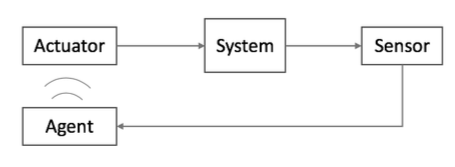
\includegraphics[width=10cm]{event.png}
 	\caption{制御系} \label{image}
\end{figure}\par
これに対するフィードバック制御を考える. 状態変数$s$を観測してアクチュエータに入力信号を送信することを「インタラクション」と呼ぶと,セルフトリガー制御では, 連続的なインタラクションは行わずに, 次のインタラクションを何秒後に行うかをエージェントが決定する. それを数式上で表すため, エージェントの制御則$\pi(s)$は2つの要素からなるベクトル値関数であるとし, 1つ目の要素はアクチュエータに送信する入力$a$,~2つ目の要素は次にインタラクションを行うまでの時間間隔$\tau~(s:秒)$を表すものとする.また, 次のインタラクションを行う時刻までは1つ前のインタラクションで送信した入力$a$を加え続けるものとする(ZOH制御).

\subsection{目標点の確認}
研究を通しての目標は「安全性を確保しながら, 最適セルフトリガー制御則$\pi^{*}$の強化学習を実現させること」である。ここで
\begin{align}
	\pi^{*} &= \argmax_{\pi}J(\pi) \label{optimal_policy}\\
	J(\pi) &= \expect_{s_0\in d_0}[V^{\pi}(s_0)] \\
	% V^{\pi}(s_0) &= \sum_{i=0}^{\infty} \gamma^i\{-s_i^{\top}Qs_i-\pi_1(s_i)^{\top}R\pi_1(s_i)+\lambda \pi_2(s_i)\} \\
	V^{\pi}(s_0) &= \sum_{i=0}^{\infty} \gamma^i C^{\pi}_i \label{value} \\
	C^{\pi}_i &= -\int_{T_i}^{T_{i+1}}s(t)^{\top}Qs(t)\textrm{d}t +\tau_ia_i^{\top}Ra_i + \lambda \tau_i, ~T_i = \sum_{l=0}^{i} \tau_l \label{reward}
\end{align}
であり,~$\pi_1, \pi_2$は$\pi$の第1,第2成分である. また, $i$はインタラクションの回数を示し, $a_i, \tau_i$はそれぞれ$i$回目のインタラクションでの方策$\pi$の出力である. \par
さて, 一般的に強化学習では, 1ステップ1ステップの行動の良し悪しを評価して方策を更新していく. 
インタラクションとインタラクションの間の区間を「インターバル」と呼ぶと, 式(\ref{value})より, この問題は各インターバルを1ステップとした強化学習問題であると考えることができる. \par
以下では方策$\pi$を$\theta$でパラメトライズし, $\theta^{*} = \argmax_{\theta}J(\pi_{\theta})$を解くことによって$\pi^{*} = \argmax_{\pi}J(\pi)$を得るものとする. 方策勾配を用いた強化学習では$\nabla_{\theta}J(\pi)$を用いて$\theta^{*}$を求める. その際方策勾配$\nabla_{\theta}J(\pi)$の近似のため, 実環境とのインタラクションによって得られたデータ組$\{s,a,r,s^{\prime}\}$を用いる. 「学習中の安全」という言葉を, 「このデータ組の収集を決められた安全領域$\mathcal{C}$の内部でのみ行うこと」と定義する.\par


\subsection{実現可能性の検証:サンプル値系での実験}
上記の目標を達成する見込みがあるのかを検証するために, サンプル値系での実験を行う. サンプル値系では,セルフトリガー制御と同様に連続的なインタラクションは行わない. セルフトリガー制御との違いは, インタラクションの間隔がエージェントによって状態$s$依存で決定するのではなく, 制御問題の設定として定数$t_{\rm{int}}$で与えられる点である.したがってサンプル値系での制御方策$\pi_{\rm{sample}}$は,アクチュエータに送信する入力信号$a$のみを出力する関数として与える.\par
サンプル値系での実験により, $t_{\rm{int}}=0.001(s)$のサンプル値系での最適方策
\begin{align}
\begin{cases}
	\pi_{\rm{sample},1} = -\argmax_{\pi_{\rm{sample}}} \displaystyle\sum_{i=0}^{\infty} \int_{it_{\rm{int}}}^{(i+1)t_{\rm{int}}}s(t)^{\top}Qs(t)\textrm{d}t + t_{\rm{int}}a_i^{\top}Ra_i \\
	a_i  = \pi_{\rm{sample}}(s(it_{\rm{int}}))
\end{cases}
\end{align}
を初期方策として,~$t_{\rm{int}}=0.002(s)$のサンプル値系での最適方策
\begin{align}
\begin{cases}
	\pi_{\rm{sample},2} = -\argmax_{\pi_{\rm{sample}}} \displaystyle\sum_{i=0}^{\infty} \int_{it_{\rm{int}}}^{(i+1)t_{\rm{int}}}s(t)^{\top}Qs(t)\textrm{d}t + t_{\rm{int}}a_i^{\top}Ra_i  \\
	a_i  = \pi_{\rm{sample}}(s(it_{\rm{int}}))
\end{cases}
\end{align}
 を学習中の安全性を満たしながら学習できるかを検証する. 

\subsection{セルフトリガー制御への発展}
前節での検証によって, インタラクション間隔を大きくしても安全強化学習を行うことが可能であることを確認できたとする. サンプル値系での制御則は入力信号$a$のみを出力する関数であったので, 入力信号$a$とインタラクション間隔$\tau$の二つの要素を出力する必要があるセルフトリガー制御の初期方策として方策$\pi_{\rm{sample},1}$をそのまま用いることはできない. \par
そこで代替策として,
\begin{align}
\begin{cases}
	\pi_1(s)=\pi_{\rm{sample},1}(s)\\
	\pi_2(s)=0.001
\end{cases} \label{pi_init}
\end{align}
とする方策$\pi_{\rm{init}}$をセルフトリガー制御の強化学習のための初期方策として用いる.

\section{安全性の定義}
\subsection{インタラクション間隔$\tau$の安全性}
ECBF(後から書きます)


\subsection{入力信号$a$の安全性}
強化学習ではデータの収集に環境とのインタラクションを行う必要がある. DDPGと呼ばれるアルゴリズムは方策オン型の強化学習とよばれ, データの収集方策に学習中の暫定最適方策を用いる. したがって,学習初期の方策では安全性が保証されないことがしばしばある. この課題を解決するために, 制御バリア関数を用いる. \par
関数$h(s)$が以下の条件を満たす時, システム(\ref{continuous})に対する制御バリア関数であるという. 
\begin{equation}
	\sup_{a\in A}\left\{\pdif{h}{s}(f(s)+g(s)a)+K(h(s))\right\} \geq 0 \label{CBF}
\end{equation}
ただし, $K(s)$はクラスK関数である.\par
さて, 2.2節にて登場した安全領域$\mathcal{C}$を
\begin{equation}
	\mathcal{C} = \left\{s \in S~|~h(s)\geq 0\right\}
\end{equation}
として与える. このとき$h(s)$が制御バリア関数であるならば, 状態$s\in C$を初期状態とした時, それ以降の全時刻において, 状態$s$が$s\in C$を満たすようにする入力が存在することを保証する. そのような入力集合は現時刻での状態$s$に依存し,
\begin{equation}
	U(s) = \left\{a \in A~|~\pdif{h}{s}(f(s)+g(s)a)+K(h(s))\geq 0\right\}, \forall s\in C
\end{equation}
としてその集合を与える.\par
学習中の安全性を確保するために, 図2のようにエージェントの出力を$U(s)$の要素に射影するレイヤーを設ける.
\begin{figure}[h]
	\centering
 	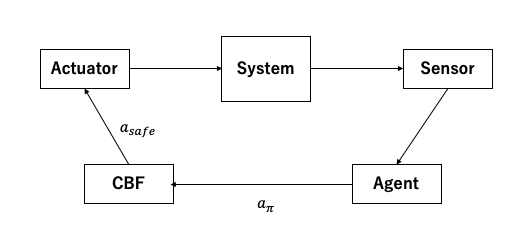
\includegraphics[width=10cm]{barrier_certificate.png}
 	\caption{制御系} \label{cbf}
\end{figure}\\
当面は, エージェントの出力$a_{\pi}$に最も近い$U(s)$の元への射影を考える.



\section{今後の方針}
\subsection{シミュレーション環境の構築}
さて, 制御バリア関数による安全性保証は連続システムに対して行われるものである. また, セルフトリガー制御則の第2成分$\tau$の出力ロジックを勾配によって更新できるように, $\tau$を連続値として扱う必要がある. しかし, コンピュータ上でシミュレーションを行うには(\ref{continuous})を時間に関して離散化を行わなくてはならない.\par
そこで, インタラクション間隔$\tau$を整数個に等間隔に分割し, その時間幅を用いて離散化を行う. この時, 離散化幅は$0.001(s)\sim 0.005(s)$になるように分割数を調整する. $\delta_t$を上から抑える理由は離散化誤差を抑えるためである. ($\tau$を)下から抑えるのは,コンピュータ上で$\frac{1}{\infty}=0$となってしまうからで, それを回避するためである.\par
ここで, 式(\ref{reward})のインターバル報酬$C^{\pi}_i$が定積分を用いて表されているため, これをシミュレーション環境で近似する手法を考える. ダイナミクス(\ref{continuous})の離散化幅$\delta_t$の離散近似システムが
\begin{equation}
	s_{t+1} = f_d(s_t, \delta_t) + g_d(s_t, \delta_t)a_t
\end{equation}
と書かれているとする. インタラクション間隔$\tau$を$N$分割した時, $\delta_t = \frac{\tau}{N}$を用いて
\begin{equation}
	C^{\pi}_i \approx -\delta_t\sum_{k=0}^{N}s_{n_i+k}^{\top}Qs_{n_i+k}+\tau_ia_i^{\top}Ra_i + \lambda \tau_i
\end{equation}
と近似する. ここで$s_{n_i}$は$i$回目のインタラクションを行った瞬間の状態変数$s(T_i)$と同じ値が代入されるものとする.\par

\subsection{サンプル値系での安全性確保ロジックの構築}
2.3節で記述した通り, $t_{\textrm{int}}$が$0.001(s)$の最適方策$\pi_{\textrm{sample},1}$を初期値として,~$0.002(s)$の最適方策$\pi_{\textrm{sample},2}$を安全強化学習できるのか検証する. 本節ではその安全性の確保方法についてもう少し掘り下げて議論する.\par
ECBFを用いることによって, 入力$a$に対するインタラクション間隔$\tau$の限界を与えることができる. その値を$\tau_{\textrm{max}}(a)$と書く. もし$\tau_{\textrm{max}}(a)<0.002$であるなら, CBFを用いて$U(s)$の元$a_{\textrm{safe}}$を選び$\tau_{\textrm{max}}(a_{\textrm{safe}})\geq0.002$となれば, 次のインタラクションまで$a_{\textrm{safe}}$を加え続けても状態変数が$\mathcal{C}$を出ていくことはない.しかし$\forall a \in U(s)$に対して$\tau_{\textrm{max}}(a)<0.002$であるなら, 次のインタラクションを$0.001(s)$後に行うことで, 安全性を確保する必要がある. ~($0.001\leq\tau_{\textrm{max}}(a)<0.002$を仮定)\par
ここまでの議論を整理すると, 「サンプル値系における安全性保証」とは「1. 入力信号の安全性,~2. サンプル間隔の安全性」を保証することになる. これらが行われることを回避する学習方法については今後検討する.


\section{セルフトリガー制御の強化学習}

\subsection{問題設定の再確認}
式\eqref{pi_init}で表される方策を初期方策として, 式\eqref{optimal_policy}で表される最適方策を学習したい. その際CBFやECBFを用いて安全性を確保する. そのために以下のものがGivenであると仮定する.
\begin{itemize}
\item 初期方策$\pi_{\textrm{init}}$ %LQRじゃ良くなさそう
\item 安全領域$\mathcal{C}$, システム\eqref{continuous} 指数制御バリア関数ECBF: $h(\mathcal{C})\geq0$
\end{itemize}

\subsection{安全確保手法}
学習中(データ収集中),~$\pi(s)=\begin{bmatrix}a & \tau\end{bmatrix}$と出力された場合を考える. ECBFを用いると, 状態$s$が安全領域$\mathcal{C}$を出ていかないための, 入力$a$を加え続けられる最大の時間$\tau_{\textrm{max}}(a)$を与えることができる. 次のインタラクションまでの時間間隔を$\min\{\tau, \tau_{\textrm{max}}(a)\}$とすることで, 安全性を確保する.

\subsection{生じると予想される課題点}
\subsubsection{$\mathcal{C}$内での経験の均一性}
方策$\pi$の正しい改善にはcriticネットワークの出力である$Q^{\pi}$の近似精度が必要不可欠である. また, DDPGはoff-policyアルゴリズムであり, 過去のデータを保存したexperience replayから作成したミニバッチを用いてcriticの更新に用いるTD誤差の計算を行う. 安全強化学習においては, $\mathcal{C}$の縁での挙動が重要であるため, 作成するミニバッチには原点付近の$(s,a)$に偏らずに, 状態変数に対して満遍なく含まれることが望ましい. 現状はexperience replayから等確率でミニバッチを作成しているので, {$\mathcal{C}$の縁での経験が少なく, 原点付近ばかりを経験していると, $\mathcal{C}$の縁付近での$Q^{\pi}$は近似精度は高くないことが予想される. \par
そこで, experience replayを原点付近の$s$と, $\mathcal{C}$の縁付近とで分けて, 均等にミニバッチを作成するのはどうかと考える. %その辺機械学習屋さんはどう考えてるのか

\subsubsection{シミュレーションの離散化による影響}
要検討

\section{セルフトリガー制御の強化学習特有の特徴に関する調査}
\subsection{準備: criticの学習速度の確認}
actorネットワークのパラメータは, 以下の方策勾配を用いて更新される.
\begin{equation}
	\nabla_{\theta^{\mu}}J(\theta^{\mu}) = \expect_{s\sim \rho^{\theta^{\mu}}}[\nabla_{\theta^{\mu}}\mu(s|\theta^{\mu})\nabla_aQ^{\theta^{\mu}(s,a)}|_{a=\mu(s|\theta^{\mu})}] \label{true_policy_gradient}
\end{equation}
ここで, ~$ \rho^{\theta^{\mu}}(s)=\int_{S}\sum_{t=0}^{\infty}\gamma^td_0(s_0)\textrm{Pr}(s_0\to s, k,  \theta^{\mu})\textrm{d}s_0$は, 割引分布という(時間割引された,全時刻における状態$s$の出現割合みたいなもの(?)). \par
式\eqref{true_policy_gradient}から, $Q^{\theta^{\mu}}$が既知でなくては, 正しい方策勾配が計算できないことがわかる. actor-criticはpolicy iterationアルゴリズムの1つであり, 方策$\mu$の更新と$Q^{\mu}$を交互に更新し続ける. DDPGではactorとcriticを1ステップにつき1回のみ更新する(つまり, criticの収束を待たずして次のステップに進む). そこで, actorを固定したときに, 実際にはcriticの学習にはどの程度のステップ数が必要なのかを知っておきたく, その実験を行った.\par
ここでは, 3つの方策$\mu_{i}$に対する$Q^{\mu}$の学習を実験する.ただし
\begin{align}
	\pi_1(s) &= \begin{bmatrix}\textrm{lqr}_{0.001}(s) \\ 0.001 \end{bmatrix} \\
	\pi_2(s) &= \begin{bmatrix}\textrm{lqr}_{0.005}(s) \\ 0.1 \end{bmatrix} \\
	\pi_3(s) &= \begin{bmatrix}\textrm a(s) \\ \tau(s) \end{bmatrix} \\
\end{align}
とする. ($\pi_3$に関しては,完全にランダムに初期化をしたNNで表現する,という意味で記載した.) \par
学習は$\theta\in[-\pi, \pi], \dot{\theta}\in[-\pi,\pi]$を50000点発生させて, $\{s, \mu_i(s), r, s^{\prime}\}$の組を保存したreplay bufferからmini batchを作成して行った. その時のloss(mini batchのTD誤差の平均)の値の変化を追った時のプロットを図\ref{critic_loss}に示す.\\
\begin{figure}[h]
	\centering
 	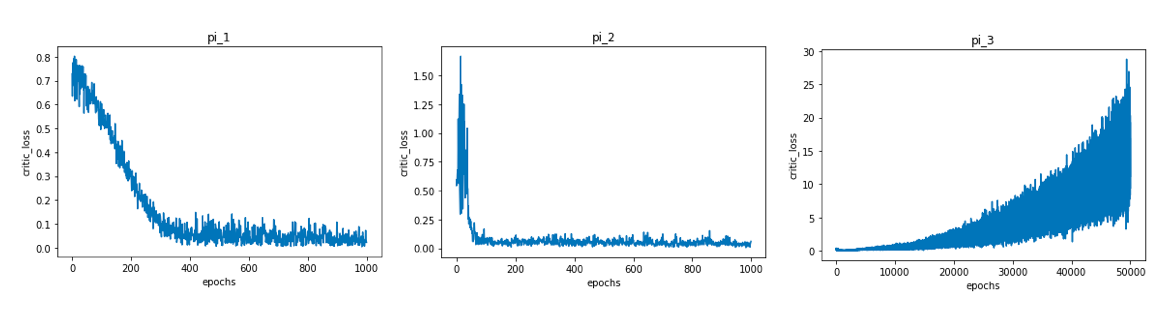
\includegraphics[width=15cm]{critic_loss.png}
 	\caption{criticの学習} \label{critic_loss}
\end{figure}\\
図\ref{critic_loss}より, 方策によって学習の様子が全く異なることが見てとれる.問題なのは$\pi_3$の学習で, これはlossが指数的に発散している. 学習率は他の2つに比べてかなり小さく取っての結果なので, 原因は最適化アルゴリズム以外にあると考える.

\subsection{方策勾配の大きさによる, 入力信号$a$と通信間隔$\tau$の学習率の考察}
図\ref{split_NN}のようにactorネットワークを, ~$a(s)$と$\tau(s)$を分離したモデルとして用いる. 
\begin{figure}[h]
	\centering
 	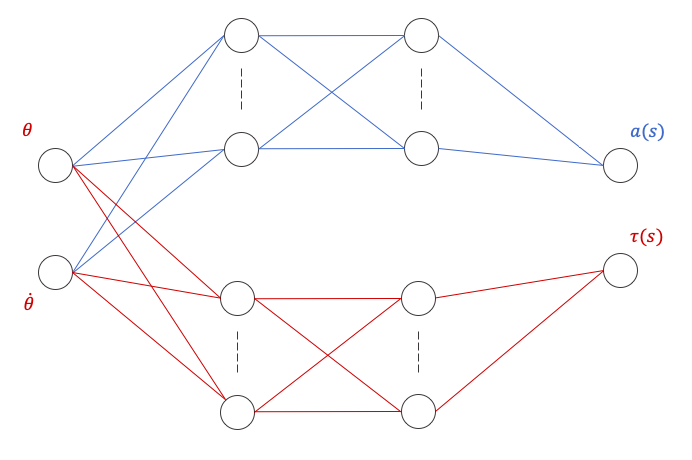
\includegraphics[width=10cm]{split_NN.png}
 	\caption{actorネットワーク} \label{split_NN}
\end{figure}\\
actorネットワークの全パラメータを$\theta^{\mu}$,~$a(s)$と$\tau(s)$を表す部分ネットワークのパラメータをそれぞれ$\theta^a, \theta^{\tau}$とする.このとき, 方策勾配$\nabla_{\theta^{\mu}}J(\theta^{\mu})$もそれぞれのパラメータが表す部分を分けて, $\nabla_{\theta^a}J(\theta^{\mu}), \nabla_{\theta^{\tau}}J(\theta^{\mu})$としたとき, パラメータの更新則は以下のようになる.
\begin{equation}
	\theta^{\mu}\gets \theta^{\mu} - \alpha_a\nabla_{\theta^a}J(\theta^{\mu}) - \alpha_{\tau}\nabla_{\theta^{\tau}}J(\theta^{\mu})
\end{equation}
研究の1つの成果物として,~$\alpha_a, \alpha_{\tau}$の理論的な大きさの設定方法について言及できればと考えている.そのため, 勾配$\nabla_{\theta^a}J(\theta^{\mu}), \nabla_{\theta^{\tau}}J(\theta^{\mu})$の大きさをそれぞれみてみる.~($\theta^{\tau}, \theta^{a}$はそれぞれ同じ長さのパラメータベクトルにしています.)\par
6.1節でcriticが収束した$\pi_1, \pi_2$について, その方策勾配$\nabla_{\theta^a}J(\theta^{\mu}), \nabla_{\theta^{\tau}}J(\theta^{\mu})$のノルムを計算すると, $\pi_1$での値は
\begin{align}
	\|\nabla_{\theta^a}J(\theta^{\mu})\| &= 66.70076 \\
	\|\nabla_{\theta^{\tau}}J(\theta^{\mu})\| &= 8.730332e-05
\end{align}
$\pi_2$での値は,
\begin{align}
	\|\nabla_{\theta^a}J(\theta^{\mu})\| &= 1.9210727 \\
	\|\nabla_{\theta^{\tau}}J(\theta^{\mu})\| &= 4.414095e-05
\end{align}
となった. このことから,~$\theta^{\tau}$の微小変化が$J$に与える影響が非常に小さいことが見てとれる. 従って, $\pi_1, \pi_2$は$\theta^{\tau}$に関するlocal maximamにある可能性が高い. 
\par
また,~$\pi_3$に関しても調べたいところであるが,正しい$Q$関数が得られていないので計算はできない. おそらく$\|\nabla_{\theta^{\tau}}J(\theta^{\mu})\|$が2つの方策の場合に対してかなり大きいのではないかと考えている. これは$\tau(s)$がどちらかに張り付くことからの予想である.\par
以上のことから, 初期方策として$\pi_1, \pi_2$を選んだ場合, ~$\tau(s)$に関しての局所最適解となっている特性と, これらの間にある方策(例えば$\pi_3$)での$\|\nabla_{\theta^{\tau}}J(\theta^{\mu})\|$が大きいという特性から,強化学習の途中で$\tau(s)$が大きく揺れてしまうことが予想される. そのため, 学習が進むにつれて減衰し, 勾配のノルムに反比例するような学習率$\alpha_{\tau}$を導入するのはどうかと考える.


\begin{thebibliography}{10}
\bibitem{ECBF}
G. Yang, C. Belta, and R. Tron. “Self-triggered Control for Safety Critical Systems Using Control Barrier Functions."  \textit{In American Control Conference (ACC) Philadelphia, USA}, 2019.
 
 \end{thebibliography}
\end{document}